% !TeX root = ../correctness-deciders.tex

\section{Bouncers}\label{sec:bouncers}

\paragraph{Acknowledgement.}  Sincere thanks to Tony Guilfoyle who initially implemented a decider for bouncers\footnote{See: \url{https://github.com/TonyGuil/bbchallenge/tree/main/Bouncers}.}.
Others have contributed to this method by producing alternative implementations (see Section~\ref{sec:bouncers-implem}) or discussing and writing the formal proof presented here: savask, Iijil, mei, Tristan Stérin (cosmo).


\begin{figure}[h!]
    \centering
    \includegraphics*[width=0.9\textwidth]{figures/bouncers/bouncers.pdf}
    \caption{Space-time diagrams (10,000 steps) of several \texttt{bbchallenge} \textit{bouncers}: (a) simple bouncer bouncing back and forth between expanding tape extremeties while writing 1s (b) bouncer with more complex alternating \textit{repeater} patterns left and right of the origin (c) unilateral bouncer with a complex \textit{wall} pattern at the origin (d) unilateral bouncer, main example used throughout this section (e) bouncer entering a repetitive bouncing pattern after $\sim$6,000 steps (bottom half of the image).}\label{fig:bouncers}
\end{figure}

\subsection{Characterising bouncers}

Intuitively, a \emph{bouncer} is a Turing machine that populates a tape with
linearly-expanding patterns, called \textit{repeaters}, possibly separated or enclosed by fixed patterns called \textit{walls}. This intuitive definition corresponds to a wide range of behaviors, from simply bouncing back and forth between the tape's expanding extremities, Figure~\ref{fig:bouncers}~(a), to complex traversal of \textit{repeater} and \textit{wall} patterns, Figure~\ref{fig:bouncers}~(b)-(d), and possibly a delayed onset of the \textit{bouncing} pattern, Figure~\ref{fig:bouncers}~(e). What we call bouncers is a generalisation of the various classes of ``Christmas trees'' used to solve $BB(4)$ \cite{Brady83}.

The goal of this section is to formally characterise bouncers and show that they do not halt, see Theorem~\ref{th:bouncers}.

\subsubsection{Directional Turing machines}\label{sec:bouncers:directionalTM}

We build on the concept of directional Turing machine introduced in Section~\ref{sec:conventions}. Directional Turing machines are an equivalent formulation of Turing machine where the machine head lives in between the tape cells and can point to the left or to the right. We choose here to treat $0^\infty$ as a unique symbol (instead of an infinite collection of 0s) and write $\overline{\Sigma} = \{0^\infty\}\cup\Sigma$, with $\Sigma=\{0,1\}$. For each Turing machine with set of state $S$ we introduce 2$|S|$ new configuration symbols (i.e.\ symbols used to describe machine configurations and not read/write symbols) denoting the machine head in two possible orientations, namely $\Delta = \{\lhead s | s\in S\}\cup\{\rhead s| s \in S\}$.

We define a \textit{tape}\footnote{Note that in the terminology of Section~\ref{sec:conventions}, the definition of a tape that we use here, where the head in part of the tape, corresponds to a (partial) TM configuration.} to be a finite word of the form $uhv$, where $u,v\in \overline{\Sigma}^*$ and $h\in\Delta$, moreover, $u$ and $v$ must have at most one occurrence of $0^\infty$ each, respectively as first symbol for $u$ or last symbol for $v$. We choose the initial tape to be $0^\infty \rhead{\text{A}} 0^\infty$. Now, we define tape rewrite rules which will be used to simulate a directional Turing machine which we fix from now on. Given two tapes $t$ and $t'$, $t\vdash t'$ will denote that a rewrite rule transforms $t$ into $t'$. Applying $\vdash$ successively $n\in\mathbb{N}$ times is written $\vdash^n$. The transitive closure of $\vdash$ (i.e.\ applying $\vdash$ \textit{some} number of times) is written $\vdash^*$.

Suppose that for $s\in S, x\in \Sigma$ we have $\delta(s,x) = (s',d,x')$ where $s'\in S, d \in \{\text{L},\text{R}\}, x' \in \Sigma$ and $\delta$ the transition function of the machine, then we define the following tape rewrite rules:


\begin{table}[h!]
    \centering
    \begin{tabular}{l|l}
        If $d = \text{L}$                               & If $d = \text{R}$ \\
        \hline
        $\begin{aligned}[t]
                 x \lhead{s}\,\,\, & \to \,\,\, \lhead{s'} x' \\
                 \rhead{s} x\,\,\, & \to \,\,\, \lhead{s'} x'
             \end{aligned}$ & $\begin{aligned}[t]
                                   x \lhead{s}\,\,\, & \to \,\,\, x' \rhead{s'} \\
                                   \rhead{s} x\,\,\, & \to \,\,\, x' \rhead{s'}
                               \end{aligned}$     \\
        \hline
    \end{tabular}\\
    \ \\ If $x=0$, also define: \\
    \begin{tabular}{l|l}
        \hline
        $\begin{aligned}[t]
                 0^\infty \lhead{s}\,\,\, & \to \,\,\, 0^\infty \lhead{s'} x'   \\
                 \rhead{s} 0^\infty\,\,\, & \to \,\,\, \lhead{s'} x'\, 0^\infty
             \end{aligned}$ & $\begin{aligned}[t]
                                   0^\infty \lhead{s}\,\,\, & \to \,\,\, 0^\infty \, x' \rhead{s'} \\
                                   \rhead{s} 0^\infty\,\,\, & \to \,\,\, x' \rhead{s'} 0^\infty
                               \end{aligned}$ \\
        \hline
    \end{tabular}\\
\end{table}

Given a tape $t=uvw$ and a word $t'=uv'w$, with $u,w\in \overline{\Sigma}^*$, $v,v' \in ( \overline \Sigma \cup \Delta)^*$, suppose that there is a rewrite rule $v \to v'$. Then $t'$ is also a tape and in this situation we write $t \vdash t'$ meaning that $t'$ is obtained from $t$ by one simulation step (i.e.\ $\vdash$ has the same meaning as for standard, non-directional, Turing machines, as introduced in Section~\ref{sec:conventions}); note that the definition is sound because, to any given tape, at most one rewrite rule applies, hence $v \to v'$ is defined uniquely and so is $t \vdash t'$. Note that the only case where $\vdash$ is not defined on a tape is if the machine halts in this configuration, i.e.\ an undefined transition is reached.

\begin{example}\label{ex:bouncer88427177}
    Consider \texttt{bbchallenge} machine\footnote{Accessible at \url{https://bbchallenge.org/88427177}} \#88,427,177 (Figure~\ref{fig:bouncers}~(d)), that has the following transition table:
    \[
        \begin{array}{l|ll}
              & 0          & 1          \\
            \hline
            A & 1\text{RB} & 1\text{LE} \\
            B & 1\text{LC} & 1\text{RD} \\
            C & 1\text{LB} & 1\text{RC} \\
            D & 1\text{LA} & 0\text{RD} \\
            E & \mbox{---} & 0LA
        \end{array}
    \]

    Given the above definitions, we will have the following rewrite rules with state A on the left-hand side:
    \begin{align*}
        0 \lhead{A}\,\,\,        & \to\,\,\, 1 \rhead{B}          \\
        \rhead{A} 0\,\,\,        & \to\,\,\, 1 \rhead{B}          \\
        1 \lhead{A}\,\,\,        & \to\,\,\, \lhead{E} 1          \\
        \rhead{A} 1\,\,\,        & \to\,\,\, \lhead{E} 1          \\
        0^\infty \lhead{A}\,\,\, & \to\,\,\, 0^\infty 1 \rhead{B} \\
        \rhead{A} 0^\infty\,\,\, & \to\,\,\, 1 \rhead{B} 0^\infty
    \end{align*}
    The other rewrite rules are those with left-hand side states B, C, D and E. Simulating the machine for 4 steps, starting from initial tape yields:
    $ 0^\infty \rhead{\text{A}} 0^\infty \;\vdash\; 0^\infty \, 1 \rhead{\text{B}} 0^\infty \;\vdash\; 0^\infty \, 1 \lhead{\text{C}} 1\, 0^\infty\ \;\vdash\; 0^\infty \, 1 \rhead{\text{C}} 1\, 0^\infty \;\vdash\; 0^\infty \, 1 1 \rhead{\text{C}} 0^\infty$. Hence, $0^\infty \rhead{\text{A}} 0^\infty \;\vdash^*\; 0^\infty \, 1 1 \rhead{\text{C}} 0^\infty$.
\end{example}

\subsubsection{Wall-repeater formula tapes}

We want to formalise the above-stated intuition that bouncers expand a tape by repeating \textit{repeater} patterns between fixed \textit{walls}, and then show that bouncers do not halt, Theorem~\ref{th:bouncers}. For this, we are going to express bouncers' tapes using regular expressions over the alphabet $\Delta \cup  \overline{\Sigma}$. Given $u\in\Sigma^*$, we abbreviate the regular expression $(u)^*$, which represents zero or more repetitions of the word $u$, as $(u)$. Also, we write $\Sigma^+ = \Sigma^* \setminus \{ \varnothing \}$. We define a \textit{wall-repeater formula tape} to be a regular expression of the form:

\begin{align}\label{math:formulaTapes}w_1(r_1)w_2(r_2)\dots w_n(r_n) w_{n+1} h w'_1(r'_1)w'_2(r'_2)\dots w'_m(r'_m) w'_{m+1}\end{align}

if the following conditions are met:
\begin{align*}
     & n,m \geq 0,                                     \\
     & h \in \Delta,                                   \\
     & r_1,\dots,r_n,r'_1,\dots,r'_m \in \Sigma^+,     \\
     & w_2,\dots,w_{n+1},w'_1,\dots,w'_m \in \Sigma^*, \\
     & w_1, w'_{m+1} \in  \overline{\Sigma}^*
\end{align*}

and, as in the definition of a tape, $w_1$ (resp. $w'_{m+1}$) either does not contain the symbol $0^\infty$ or it starts with it (resp. ends with it). Patterns $w_i, w'_j$ are called \textit{walls} and can be empty, while the \textit{repeaters}, $r_i, r'_j$ must be nonempty. Note that we allow $n=m=0$, hence a usual tape is also a wall-repeater formula tape. For the rest of this section, we abbreviate wall-repeater formula tapes as \textit{formula tapes}.

Given a formula tape $f$ let $\mathcal{L}(f)$ denote the language described by $f$, i.e.\ the set of tapes that match it.
% Given two formula tapes $f$ and $f'$ we will say that $f'$ is a \textit{special case} of $f$ if $\mathcal{L}(f') \subseteq \mathcal{L}(f)$. Note that it is equivalent to saying that $f'$ can be obtained from $f$ by replacing subwords of the form $(r), r\in\Sigma^*\setminus\{\varnothing\}$ by $r^n(r)r^m$ for some $n,m\geq 0$.

\begin{example}\label{ex:formulaTapes}
    Consider the formula tape $f = 0 \rhead{\text{D}} (01)$. We have $\mathcal{L}(f) = \{0\rhead{\text{D}},0\rhead{\text{D}}01,0\rhead{\text{D}}0101,\dots\}$. Consider the formula tape $f'=0^\infty(111)1110 \lhead{\text{A}} 010101(01)10^\infty$. Then: $0^\infty 1110 \lhead{A} 01010110^\infty$, $0^\infty 1111110 \lhead{A} 01010110^\infty$, and $0^\infty 1110 \lhead{A} 0101010110^\infty$ are three elements of $\mathcal{L}(f')$.
\end{example}

% \paragraph*{Aligning formula tapes.}  



% Consider the formula tape $f = 0^\infty 101(11)0 \rhead{\text{D}} 10(100)110^\infty$. The following formula tape $\tilde{f} = 0^\infty 10(11)10 \rhead{\text{D}} 101(001)10^\infty$ describes the same language as $f$, i.e.\ $\mathcal{L}(f) = \mathcal{L}(\tilde{f})$.

\paragraph*{Extending $\vdash$ to formula tapes: \textit{shift rules}.} We wish to extend the Turing machine step relation $\vdash$ (see Section~\ref{sec:bouncers:directionalTM}) to formula tapes. This is quite straightforward when the formula tape's head is pointing at a symbol of a wall (one of the $w_i, w'_j$ in \eqref{math:formulaTapes}): we simply apply a standard Turing machine step, leaving the definition of $\vdash$ unchanged.

However, we need to handle the case where the head is pointing at a repeater (one of the $r_i, r'_j$ in \eqref{math:formulaTapes}). Suppose that for some $u\in\Sigma^*$ and $r,\tilde{r}\in\Sigma^+$ and some state $s\in S$ we have $u \rhead{s} r \vdash^* \tilde{r} u \rhead{s}$. Then, for any $n\geq 0$, we have $u \rhead{s} r^n \vdash^* \tilde{r}^n u \rhead{s}$. This motivates the definition of
(right) \textit{shift rules}, rewrite rules for formula tapes, which rewrite a subword $u \rhead{s}(r)$ into $(\tilde{r})u\rhead{s}$, denoted $u \rhead{s}(r) \to (\tilde{r})u\rhead{s}$. Similarly, left shift rules are of the form $(r)\lhead{s}u \to \;\lhead{s}u(\tilde{r})$ given that $r\lhead{s}u \vdash^* \;\lhead{s}u\tilde{r}$. Note that repeaters $r$ and $\tilde{r}$ of a shift rule necessarily have the same size since $\vdash$ preserves tapes' size.

Hence, we have two cases to consider for defining $\vdash$ on the following formula tape $f$ (as defined in~\eqref{math:formulaTapes}):
$$f = w_1(r_1)w_2(r_2)\dots w_n(r_n) w_{n+1} h w'_1(r'_1)w'_2(r'_2)\dots w'_m(r'_m) w'_{m+1}$$

\begin{enumerate}
    \item (Usual step) If $h$ points to nonempty $w_{n+1}$ or $w'_1$, then $f \vdash \alpha \tilde{w}_{n+1} \tilde{h} \tilde{w}'_1\beta$ if $w_{n+1} h w'_1 \vdash \tilde{w}_{n+1} \tilde{h} w'_1$, $\tilde{w}_{n+1}, \tilde{w} \in \Sigma^*$, $\tilde{h} \in \Delta$, and $\alpha, \beta$ the above uniquely-defined beginning and ending of $f$. As for tapes, $\vdash$ is undefined if $w_{n+1} h w'_1$ corresponds to a halting configuration (i.e.\ undefined transition).
          % Using \eqref{math:formulaTapes}, write as $f=\alpha w_{n+1} h w'_1\beta$, with $\alpha$ (resp. $\beta$) the uniquely-defined beginning (resp.ending) of the formula tape $f$. Then, $f \vdash \alpha \tilde{w}_{n+1} \tilde{h} \tilde{w}'_1 \beta = f'$ if $w_{n+1} h w'_1 \vdash \tilde{w}_{n+1} \tilde{h} \tilde{w}'_1$ with $\tilde{w}_{n+1}, \tilde{w} \in \Sigma^*$ and $\tilde{h} \in \Delta$.
    \item (Shift rule) Two cases:
          \begin{enumerate}

              \item Right shift rule. If $h=\;\rhead{s\in S}$ and $w'_1$ is empty, consider the set of shift rules $\mathcal{R} = \{ u \rhead{s}(r'_1) \to (\tilde{r})u\rhead{s} \; | \; \tilde{r}\in\Sigma^+,\; u\in\Sigma^* \text{ is a suffix of } w_{n+1}\}$. If $\mathcal{R}$ is not empty then apply the right shift rule of $\mathcal{R}$ with smallest $u$ (possibly empty), call the new formula $f'$, and we have $f \vdash f'$. If $\mathcal{R}$ is empty, $\vdash$ cannot be applied to $f$.
              \item Left shift rule. If $h=\;\lhead{s\in S}$ and $w_{n+1}$ is empty, consider the set of shift rules $\mathcal{R} = \{ (r_{n})\lhead{s}u \to \;\lhead{s}u(\tilde{r}) \; | \; \tilde{r}\in\Sigma^+,\; u\in\Sigma^* \text{ is a prefix of } w'_{1}\}$. If $\mathcal{R}$ is not empty then apply the left shift rule of $\mathcal{R}$ with smallest $u$ (possibly empty), call the new formula $f'$, and we have $f \vdash f'$. If $\mathcal{R}$ is empty, $\vdash$ cannot be applied to $f$.

          \end{enumerate}

\end{enumerate}

From the above definition of $\vdash$ on a formula tape $f$, it is clear that (i) for usual tapes our new definition of $\vdash$ coincides with the old one, (ii) there is at most one formula tape $f'$ such that $f \vdash f'$, and (iii) the only cases where $\vdash$ is not defined on a formula tape are when the machine halts (usual step case) or no shift rule applies (shift rule case). Moreover, we get the following result:

\begin{lemma}\label{lem:vdashFormulaTapes} Let $f$ and $f'$ be formula tapes with $f \vdash f'$. Then, for all $t \in \mathcal{L}(f)$, there exists some $t' \in \mathcal{L}(f')$ such that $t \vdash^* t'$.
\end{lemma}
\begin{proof}
    If $f'$ follows from $f$ by a usual step, then applying one usual step to $t$ yields $t'\in\mathcal{L}(f')$. If $f'$ follows from $f$ by a shift rule, we apply several steps to $t$ (as many as there in the shift rule) to obtain $t' \in \mathcal{L}(f')$.
\end{proof}

% Ambiguity in shift rule application:
% If 1 s> (r) -> (1111) 1 s> and there is a 1 to the left of the initial u=1 then, we also have 11 s> (r) -> (1111) 11 s>

\begin{example}\label{ex:shiftRules}
    Taking the machine of Example~\ref{ex:bouncer88427177}, we have the right shift rule $0 \rhead{\text{D}}(01) \to (11)0\rhead{\text{D}}$. Indeed, this is because: $0 \rhead{\text{D}}01 \vdash 0\lhead{\text{A}}11 \vdash 1\rhead{\text{B}}11 \vdash 11\rhead{\text{D}}1 \vdash 110\rhead{\text{D}}$, hence $0 \rhead{\text{D}}01 \vdash^* 110\rhead{\text{D}}$, giving the shift rule. Consider the tape formula of previous Example~\ref{ex:formulaTapes}: $f' = 0^\infty(111)1110 \lhead{\text{A}} 010101(01)10^\infty$. We have $f' \vdash^{13} 0^\infty (111)1111110110 \rhead{\text{D}} (01) 10^\infty$, at this point the head points to a repeater and the set of applicable right shift rules is $\mathcal{R} = \{ 0 \rhead{\text{D}}(01) \to (11)0\rhead{\text{D}},\; 10 \rhead{\text{D}}(01) \to (11)10\rhead{\text{D}},\; 110 \rhead{\text{D}}(01) \to (11)110\rhead{\text{D}}\}$, and following the definition of $\vdash$, we apply $0 \rhead{\text{D}}(01) \to (11)0\rhead{\text{D}}$ as it has the smallest left-hand side, giving: $0^\infty (111)111111011(11)0 \rhead{\text{D}} 10^\infty$.

\end{example}

\paragraph*{Aligning formula tapes.} One last tool that we need before characterising bouncers and proving that they do not halt (Theorem~\ref{th:bouncers}) is formula tape \textit{alignment} (Definition~\ref{def:alignment}): sometimes it is necessary to rewrite a formula tape in an equivalent, \textit{aligned} form in order for any shift rules to apply.

\begin{definition}[Alignment operator]\label{def:alignment}
    Take a formula tape, as given in~\eqref{math:formulaTapes}: $$f = w_1(r_1)w_2(r_2)\dots w_n(r_n) w_{n+1} h w'_1(r'_1)w'_2(r'_2)\dots w'_m(r'_m) w'_{m+1}$$

    The alignment operator $f \mapsto \mathcal{A}(f)$ moves repeaters away from the head $h$ by repeatedly applying any of the following rules until none apply anymore:
    \begin{enumerate}
        \item Replace $(r'_{j})v$ with $v(r)$ in $f$, if $r'_j v = v r$ with $v$ a nonempty prefix of $w'_{j+1}$, $r\in\Sigma^+$, and $1 \leq j \leq m$.

        \item Replace $v(r_{i})$ with $(r)v$ in $f$, if $v r_i = r v$ with $v$ a nonempty suffix of $w_{i}$, $r\in\Sigma^+$, and $1 \leq i \leq n$.
    \end{enumerate}

    Clearly, the order application of these rules does not matter, i.e.\ $\mathcal{A}$ is well-defined, and $\mathcal{A}(\mathcal{A}(f)) = \mathcal{A}(f)$.
\end{definition}



\begin{lemma}\label{lem:sameLanguage} For any formula tape $f$, $\mathcal{L}(\mathcal{A}(f)) = \mathcal{L}(f)$, i.e.\ both $f$ and $\mathcal{A}(f)$ represent the same set of tapes.
\end{lemma}

\begin{proof}
    Consider an alignment rule as in case (1) of Definition~\ref{def:alignment}: replacing $(r'_{j})v$ with $v(r)$ if $r'_j v = v r$. Then, for all $n\in\mathbb{N},\; {r'_j}^n v = v r^n$, hence $(r'_{j})v$ and $v(r)$ describe the same language: $\mathcal{L}((r'_{j})v) = \mathcal{L}(v(r))$. Same for case (2) and for multiple applications of (1) and (2) in any order, hence we have $\mathcal{L}(\mathcal{A}(f)) = \mathcal{L}(f)$.
\end{proof}

\begin{example}\label{ex:alignment}
    Take $f=0^\infty(111)1111\rhead{\text{B}}(01)01010110^\infty$ for the machine given in Example~\ref{ex:bouncer88427177}. One can verify that no right shift rule applies to $f$ hence $\vdash$ does not apply to $f$. However, we have $ \mathcal{A}(f)=0^\infty(111)1111\rhead{B}010101(01)10^\infty$, $\mathcal{L}(\mathcal{A}(f)) = \mathcal{L}(f)$, and we can apply $\vdash$ to $ \mathcal{A}(f)$ by performing usual steps: $ \mathcal{A}(f) \vdash^{12} 0^\infty(111)1111110110 \rhead{D} (01)10^\infty$ and now the shift rule of Example~\ref{ex:shiftRules} can apply, giving $0^\infty(111)111111011(11)0 \rhead{\text{D}} 10^\infty$.
    Another alignment example is $f=0^\infty 101(11)0 \rhead{\text{D}} 10 (100) 11 0^\infty$ for which $\mathcal{A}(f) = 0^\infty 10(11)10 \rhead{\text{D}} 101(001)10^\infty$.
\end{example}





\begin{remark}[Alignment never hurts]
    Example~\ref{ex:alignment} shows that alignment (which preserves the set of recognised tapes) can allow to run a shift rule on $f'$ with $\mathcal{A}(f) \vdash^* f'$ when no shift rule was applicable directly to $f$. In fact, one can show that the alignment operator can only \textit{increase} the number of applicable shift rules: if a shift rule is applicable to $f$ then a shift rule applicable to $f'$ with $\mathcal{A}(f) \vdash^* f'$ can always be constructed.
\end{remark}

Given two formula tapes $f$ and $f'$ we will say that $f'$ is a \textit{special case} of $f$, if $\mathcal{A}(f')$ can be obtained from $\mathcal{A}(f)$ by replacying subwords of the form $(r)$ by $r^n(r)r^m$ for some $n,m\geq 0$ and $r\in\Sigma^+$. Note that because of alignment, $n=0$ (resp. $m=0$) if $(r)$ is to the left (resp. to the right) of the head. If $f$ is a special case of $f'$ then $\mathcal{L}(f) \subseteq \mathcal{L}(f)$, the converse is open but conjectured true\footnote{See \url{https://discuss.bbchallenge.org/t/186}.} (under additional assumptions).

We finally get to the main result of this section, which characterises bouncers formally -- a bouncer is any machine to which Theorem~\ref{th:bouncers} applies:

\begin{theorem}[Bouncers]\label{th:bouncers}
    Assume we are given some Turing machine and suppose there exists a tape $t$ and some wall-repeater formula tapes $f_0,\dots,f_n, n\geq 1$, such that $0^\infty \rhead{\text{A}} 0^\infty \vdash^* t$ where $t \in \mathcal{L}(f_0)$, and $\mathcal{A}(f_i) \vdash f_{i+1}$ for $i=0,\dots,n-1$. If $f_n$ is a special case of $f_0$, then the Turing machine does not halt.
\end{theorem}

\begin{proof}
    It follows from Lemma~\ref{lem:vdashFormulaTapes} and Lemma~\ref{lem:sameLanguage} that there exists tapes $t_0, \dots, t_n$, such that $t_0 = t$ and $t_i\in \mathcal{L}(f_i)$ for $0 \leq i \leq n$, and $t_i \vdash^* t_{i+1}$ for $0 \leq i < n$, giving $t_0 \vdash^* t_n$. Since $f_n$ is a special case of $f_0$, we have $\mathcal{L}(\mathcal{A}(f_n)) \subseteq \mathcal{L}(\mathcal{A}(f_0))$, and using Lemma~\ref{lem:sameLanguage}, we have $\mathcal{L}(f_n) \subseteq \mathcal{L}(f_0)$ and thus, $t_n \in \mathcal{L}(f_0)$, we can repeat this construction indefinitely and yield an infinite sequence of tapes $(t_n)_{n\in\mathbb{N}}$ such that $t \vdash^* t_i$ for all $i\in\mathbb{N}$: the machine does not halt.
\end{proof}

\begin{example}\label{ex:bouncerTheory}
    Theorem~\ref{th:bouncers} applies to the machine of Example~\ref{ex:bouncer88427177}, illustrated in Figure~\ref{fig:bouncers}~(d), used in our series of examples for this section. Indeed, we have $0^\infty \rhead{\text{A}} 0^\infty \vdash^{64} 0^\infty 11111101100 \rhead{\text{D}} 0^\infty$, this tape, $t=0^\infty \vdash^{64} 0^\infty 11111101100 \rhead{\text{D}} 0^\infty$ is in the language the following formula tape:
    $$f_0 = 0^\infty (111)1110(11)00\rhead{\text{D}}0^\infty$$
    At this point, and for the next 25 usual steps alignment does not affect the formulas, and we get: $$f_{25} = 0^\infty (111) 1110 (11) \lhead{\text{A}} 01010110^\infty$$
    One shift rule gives:
    $$ f_{26} = 0^\infty (111) 1110  \lhead{\text{A}} (01) 01010110^\infty$$
    After alignment:
    $$ \mathcal{A}(f_{26}) = 0^\infty (111) 1110  \lhead{\text{A}} 010101(01)10^\infty$$
    From there, $\mathcal{A}(f_{26}) \vdash f_{27}$ with:
    $$ f_{27} = 0^\infty (111) 1111  \rhead{\text{B}} 010101(01)10^\infty$$
    After 12 usual steps, not affected by alignment, we arrive at:
    $$f_{39} = 0^\infty (111)1111110110\rhead{\text{D}}(01)10^\infty$$
    One shift rule gives:
    $$f_{40} = 0^\infty (111)111111011(11)0\rhead{\text{D}}10^\infty$$
    Aligning gives:
    $$\mathcal{A}(f_{40}) = 0^\infty (111)1111110(11)110\rhead{\text{D}}10^\infty$$
    Finally, from there $\mathcal{A}(f_{40}) \vdash f_{41}$ with one usual step:
    $$f_{41} =\mathcal{A}(f_{41}) = 0^\infty (111)1111110(11)1100\rhead{\text{D}}0^\infty$$

    Now, $f_{41}$ is a special case of $f_{0}$ because $\mathcal{A}(f_{41})$ differs from $f_0=\mathcal{A}(f_0)$ only by including one repetition of repeaters $(111)$ and $(11)$ in the walls directly to their right. The assumptions of Theorem~\ref{th:bouncers} hold and our Turing machine is a bouncer: it does not halt.
\end{example}

\begin{remark}
    Both Cyclers (Section~\ref{sec:cyclers}) and Translated Cyclers (Section~\ref{sec:translated-cyclers}) are special cases of bouncers, as they satisfy Theorem~\ref{th:bouncers}.
\end{remark}


\subsubsection{Linear-quadratic growth}

Theorem~\ref{th:bouncers} characterises bouncers but we lack a practical criterion for recognising a bouncer from its sequence of successive tapes starting from $0^\infty \rhead{\text{A}} 0^\infty$. We make a step in that direction by showing that if a bouncer is not a cycler (Section~\ref{sec:cyclers}), we can expect to see tapes of the form $w_1 r_1^n w_2 r_2^n \dots w_m r_m^n w_{m+1}$ for some $m\in\N$ and for all successive $n\in\mathbb{N}$ as a subsequence of the sequence of all tapes visited by the bouncer.

We define \textit{record-breaking tapes} to be tapes where the head is pointing at $0^\infty$, i.e.\ tapes of the form $0^\infty u \rhead{s} 0^\infty$ or $0^\infty \lhead{s} u 0^\infty$ with $u\in\Sigma^*$. Give a tape $t$, we call $\mathcal{S}(t) \in \Sigma^*$ the \textit{headless} version of $t$ which is the tape without head and $0^\infty$ symbols. The \textit{length} of a tape $t$ is defined as the number of symbols in $\mathcal{S}(t)$. We also introduce headless formula tapes: $\mathcal{S}(f)$ is $f$ without head and $0^\infty$ symbols. Also, we extend the alignment operator $\mathcal{A}$ (Definition~\ref{def:alignment}) to headless formula tapes by performing right-alignment. We denote an infinite sequence $u_0, u_1, \dots u_n, \dots$ with $n\in\N$ by $(u_n)_{n\in\N}$. We define the difference operator $D: \N^\N \to \N^\N$ via $D((u_n)_{n\in\N})=(u_{n+1}-u_{n})_{n\in\N}$.

Bouncers will grow their tape such that we can extract a subsequence of record-breaking tapes of the form $w_1 r_1^n w_2 r_2^n \dots w_m r_m^n w_{m+1}$ with length in arithmetic progression and time steps in quadratic progression:

\begin{theorem}[\textit{Linear-quadratic growth}]\label{th:linquad}
    Let $M$ be a bouncer Turing machine, i.e.\ it satisfies Theorem~\ref{th:bouncers} for some formula tape. Call $(t_n)_{n\in\N}$ the sequence of tapes that it visits starting from $t_0 = 0^\infty \rhead{\text{A}} 0^\infty$. Call $l_n$ the length of $t_n$ and suppose that $\Lim{n\to\infty} l_n = +\infty$, i.e.\ $M$ is not a cycler. Then, there is an integer $m \geq 1$ and $w_1, \dots, w_{m+1} \in \Sigma^*$ and $r_1, \dots, r_{m} \in \Sigma^+$, and $g: \mathbb{N} \to \mathbb{N}$ with $g(n) \geq n$ for all $n\in\N$ that extracts a subsequence of $(t_n)_{n\in\N}$ such that:

    \begin{enumerate}
        \item There is a formula tape $f$ with head pointing at $0^\infty$ that solves the bouncer according to Theorem~\ref{th:bouncers} and with $\mathcal{S}(f) = w_1 (r_1) w_2 (r_2) \dots w_m (r_m) w_{m+1} $.
        \item All tapes $t_{g(n)}$ are record-breaking with the same head state and pointing-direction.
        \item $\mathcal{S}(t_{g(n)})=w_1 r_1^n w_2 r_2^n \dots w_m r_m^n w_{m+1}$ for all $n\in\N$.

        \item $(l_{g(n)})_{n\in\N}$ is an arithmetic progression, i.e.\ $D((l_{g(n)})_{n\in\N}) = (K)_{n\in\N}$ for some constant $K\in\N$.
        \item $(g(n))_{n\in\N}$ is a quadratic progression, i.e.\ $D(D((g(n))_{n\in\N})) = (K')_{n\in\N}$ for some constant $K'\in\N$.
    \end{enumerate}
\end{theorem}

\begin{proof}
    Because $M$ is a bouncer, there is a formula tape (See~\eqref{math:formulaTapes}): $$\tilde{f} = 0^\infty\tilde{w}_1(\tilde{r}_1)\tilde{w}_2(\tilde{r}_2)\dots \tilde{w}_n(\tilde{r}_n) \tilde{w}_{n+1} h \tilde{w'}_1(r'_1)\tilde{w'}_2(\tilde{r'}_2)\dots \tilde{w'}_m(\tilde{r'}_m) \tilde{w'}_{m+1}0^\infty$$

    With $h\in\Delta$, $\tilde{w}_i, \tilde{w}'_j \in \Sigma^*$, $\tilde{r}_i, \tilde{r}_j \in \sigma^+$.

    There is also $\tilde{f}_0 = \tilde{f}$, $\tilde{f}_1, \dots \tilde{f}_k$ with $k \in \N$ such that $\mathcal{A}(\tilde{f}_i) \vdash \tilde{f}_{i+1}$ for $0 \geq i < k$ and $\tilde{f}_k$ is a special case of $\tilde{f}_0$.

    Because $\Lim{n\to\infty} l_n = +\infty$, there must be $0 \leq j < k$ such that the head of $\tilde{f}_{j}$ is pointing to $0^\infty$ (otherwise the tape would never grow). Hence, without loss of generality, by rotating the sequence of formula tapes, we can assume that the head of $\tilde{f}_{0}=\tilde{f}$ is pointing at $0^\infty$, so does the head of $\tilde{f}_k$, by special case. Furthermore, we can assume that each wall preceding a repeater in $\tilde{f}_k$ is bigger than its corresponding wall in $\tilde{f}_0$, otherwise the repeater is useless (it never grows) and can be merged into its preceding wall in both formulas.

    Hence, from the above and because $\tilde{f}_k$ is a special case of $\tilde{f}_0$, renaming the walls' and repeaters' symbols we get:
    \begin{align*}
        \mathcal{A}(\mathcal{S}(\tilde{f}))   & = \tilde{w}_1(\tilde{r}_1)\tilde{w}_2(\tilde{r}_2)\dots \tilde{w}_n(\tilde{r}_n) \tilde{w}_{n+1}                                                    \\
        \mathcal{A}(\mathcal{S}(\tilde{f}_k)) & = \tilde{w}_1\tilde{r}_1^{m_1}(\tilde{r}_1)\tilde{w}_2\tilde{r}_2^{m_2}(\tilde{r}_2)\dots \tilde{w}_n\tilde{r}_2^{m_n}(\tilde{r}_n) \tilde{w}_{n+1}
    \end{align*}

    With $m_1, \dots, m_n \geq 1$.

    From Theorem~\ref{th:bouncers}, we know that the machine reaches a tape $t\in\mathcal{L}(\tilde{f})$. We can furthermore suppose that the machine will reach the tape $\tilde{w}_1\tilde{w}_2\dots \tilde{w}_n \tilde{w}_{n+1}$ as we simply have to redefine our walls if it reaches some tape with more initial repetitions of the repeaters instead. Hence, by successive simulation and alignment of the formula tape $f$ with same head as $\tilde{f}_0$  such that $\mathcal{A}(\mathcal{S}(f)) = \tilde{w}_1(\tilde{r}_1^{m_1})\tilde{w}_2(\tilde{r}_2^{m_2})\dots \tilde{w}_n(\tilde{r}_2^{m_n}) \tilde{w}_{n+1}$, renamed as $\mathcal{A}(\mathcal{S}(f)) = w_1(r_1)w_2(r_2)\dots w_n(r_2) w_{n+1}$, we are assured to solve the bouncer (i.e.\ reach a special case) and, by continuing simulation, to generate an infinite subsequence of reached tapes of the form $\mathcal{S}(t_{g(n)})=w_1 r_1^n w_2 r_2^n \dots w_m r_m^n w_{m+1}$ for all $n\in\N$ and for $g: \N \to \N$ some extraction function with $g(n) \geq n$ for all $n \in \N$.

    All such tapes are record-breaking with same head, by construction. Hence, we proved points 1-3. Point 4 comes easily because from the expression we have for $t_{g(n)}$, we get $l_{g(n+1)} - l_{g(n)} = |r_1| + \dots |r_m| = K$, which is constant. Concerning point 5, we have $g(n+1)-g(n)$ = $M + ns_1 + ns_2 + \dots ns_m$, with $M\in\N$ a constant related to processing walls and $s_1, \dots s_m \in \N$ the constant time needed to run the shift rule associated to each repeater $r_1 \dots r_m$. Hence we get $D(D((g(n))_{n\in\N})) = s_1+\dots + s_n = K'$, which is constant.


\end{proof}

% with formula tape $f=0^\infty 111(111)01111(11)\rhead{\text{C}}0^\infty$, which is another formula tape that decides the bouncer (different from the one given in Example~\ref{ex:bouncerTheory}),

\begin{example}\label{ex:linquad}
    Using the machine of Example~\ref{ex:bouncer88427177} used in the previous section, we have:
    \begin{align*}
        0^\infty \rhead{\text{A}} 0^\infty & \vdash^{37} 0^\infty 111\; 01111 \rhead{\text{C}} 0^\infty                                 & g(0) = 37,\; l_{37} = 11   \\
                                           & \vdash^{39}   0^\infty111\; 111 \;01111 \;11\rhead{\text{C}}0^\infty                       & g(1) = 76,\; l_{76} = 16   \\
                                           & \vdash^{45}   0^\infty111\; 111\;111\; 01111\; 11\; 11 \rhead{\text{C}}0^\infty            & g(2) = 121,\; l_{121} = 21 \\
                                           & \vdash^{51}   0^\infty111\; 111\;111\; 111\; 01111\; 11\; 11\; 11 \rhead{\text{C}}0^\infty & g(3) = 172,\; l_{172} = 26 \\
    \end{align*}
    Each of these tapes are record-breaking using the same head $\rhead{\text{C}}$. Then, in this finite sample, $l_{g(0)},...,l_{g(3)}$ is in arithmetic progression with first difference $K=5$ and $g(0), ..., g(3)$ is in quadratic progression with second difference $K'=6$.

    In general, we get:
    $$0^\infty \rhead{\text{A}} 0^\infty  \vdash^{g(n)} 0^\infty 111\; (111)^n\; 01111 (11)^n\; \rhead{\text{C}} 0^\infty   \quad g(n) = 3n^2 + 36n + 37,\; l_{g(n)} = 5n+11$$

    This general expression can be verified by simulating (and aligning) the formula tape $f=111(111)01111(11)\rhead{\text{C}}0^\infty$ until it reaches a special case, which solves the bouncer (Theorem~\ref{th:bouncers}).

\end{example}
\newpage
\subsection{Deciding bouncers in practice}

In this section, we use the theory presented above in order to give a practical and efficient algorithm for deciding bouncers.

\subsubsection{Formula tape fitting}

Theorem~\ref{th:linquad} assures us that, in the sequence of successive tapes of a bouncer, we'll always find a subsequence where all repeaters' repetitions successively increase by one. Given such a subsequence, we are left with the task of fitting an appropriate formula tape. It turns out that only 3 successive tapes $(t_0,t_1,t_2)$, with at least one repetition of each repeater in the first tape, are enough to fit a formula tape efficiently using a greedy algorithm which recursively constructs the left-most wall using the biggest common prefix of $t_0, t_1$ and $t_2$ and then fits as left-most repeater the longest prefix $r$ of $t_1$ such that $rr$ is a prefix of $t_2$:

\begin{algorithm}
    \caption{Greedy formula tape fitting algorithm {\sc Fit-FormulaTape}}\label{alg:greedy-formula-tape-fitting}
    \begin{algorithmic}[1]

        \Procedure{\textbf{FormulaTape} {\sc Fit-FormulaTape}}{\textbf{Word} t0, \textbf{Word} t1, \textbf{Word} t2}

        \If{t0.\textbf{empty}() \&\& t1.\textbf{empty}() \&\& t2.\textbf{empty}()}
        \State \Return \textbf{FormulaTape}::\textbf{empty}()

        \EndIf
        \State
        \If{t0.\textbf{len}() $>$ 0 \&\& t1.\textbf{len}() $>$ 0 \&\& t2.\textbf{len}() $>$ 0 \&\& t0[0] == t1[0] \&\& t1[0] == t2[0]}
        \State \Return \textbf{FormulaTape}::\textbf{symbol}(t0[0]).\textbf{concat}(\Call{{\sc Fit-FormulaTape}}{t0[1:], t1[1:], t2[1:]})
        \EndIf
        \State
        \State
        \textbf{uint} longest\_prefix\_size = \textbf{get\_longest\_prefix\_size}(t1, t2)
        \State
        \For{l = longest\_prefix\_size; k $\geq$ 1; k -= 1 }

        \If{2*l $<$ t2.\textbf{len}() \&\& t2[:l] == t2[l:2*l] }
        \State \Return \textbf{FormulaTape}::\textbf{repeater}(t2[:l]).\textbf{concat}(\Call{{\sc Fit-FormulaTape}}{t0, t1[l:], t2[2*l:]})
        \EndIf

        \EndFor
        \State
        \State \textbf{raise} \textbf{Failure}
        \EndProcedure
    \end{algorithmic}
\end{algorithm}

\begin{remark}
    In Algorithm~\ref{alg:greedy-formula-tape-fitting}, we assume that we are given a \textbf{FormulaTape} construct (see Equation~\eqref{math:formulaTapes}) that we use for headless formula tapes and a function \textbf{get\_longest\_match\_size} which returns the size of the longest prefix of two words. Furthermore, for an array \texttt{a}, we use the notation \texttt{a[b:e]} to mean the slice of this array between indices \texttt{b} and \texttt{e}, excluding \texttt{e}.
\end{remark}

% \begin{lemma}\label{lem:greedy}
%     Let there be 3 words $t_0, t_1, t_2 \in \Sigma^*$, and an integer $m\in\N$ and $w_1, w_2 \in \Sigma^*$ and $r \in\Sigma^+$ the longest word such that $t_0 = w_1\; r\; w_2$, and $t_1 = w_1\; rr\; w_2$ and $t_2 = w_1\; rrr\; w_2$, then we have:
%     \setlength{\columnsep}{-6.5cm}
%     \begin{multicols}{3}
%         \noindent
%         \begin{align*}
%             t_0 & = w_1\; r\; w_2   \\
%             t_1 & = w_1\; rr\; w_2  \\
%             t_2 & = w_1\; rrr\; w_2 \\
%             f   & = \varnothing
%         \end{align*}
%         \begin{align*}
%              &                                                                   \\
%             \to_{\text{Algorithm~\ref{alg:greedy-formula-tape-fitting} goes to}} \\
%              &                                                                   \\
%              &
%         \end{align*}
%         \begin{align*}
%             t_0 & = \varnothing              \\
%             t_1 & = \varnothing              \\
%             t_2 & = \varnothing              \\
%             f   & = \mathcal{A}(w_1r(r) w_2)
%         \end{align*}
%     \end{multicols}
%     Meaning that Algorithm~\ref{alg:greedy-formula-tape-fitting} function call {\sc Fit-FormulaTape}($t_0$, $t_1$, $t_2$) does not raise failure and returns the right-aligned headless formula tape $\mathcal{A}(w_1r(r) w_2)$.
% \end{lemma}
% \begin{proof}




% \end{proof}


\begin{theorem}[Greedy formula tape fitting]\label{th:greedy-formula-tape-fitting}
    Let there be 3 words $t_0, t_1, t_2 \in \Sigma^*$, and an integer $m>0$ and $w_1, \dots w_{m+1} \in \Sigma^*$ and $r_1, \dots, r_m \in\Sigma^+$ the longest repeaters such that:
    \begin{align*}
        t_0 & = w_1\; r_1\; \dots w_m\; r_m\; w_{m+1}               \\
        t_1 & = w_1\; r_1r_1\; \dots w_m\; r_m r_m\; w_{m+1}        \\
        t_2 & = w_1\; r_1 r_1 r_1 \dots w_m\; r_m r_m r_m\; w_{m+1}
    \end{align*}
    Then Algorithm~\ref{alg:greedy-formula-tape-fitting} ran on {\sc Fit-FormulaTape}($t_0$, $t_1$, $t_2$) does not raise failure and returns the right-aligned headless formula tape $\mathcal{A}(w_1 r_1 (r_1) \dots w_m r_m (r_m) w_{m+1})$.

\end{theorem}
\begin{proof}
    Let's first prove the case $m=1$ and write $r_1 = r$.
    Notation: if a word $w\in\Sigma^*$ is not empty we use the notation $w[0]$ to mean the first symbol of $w$. Using the case of Algorithm~\ref{alg:greedy-formula-tape-fitting}, line 10, we get:
    \setlength{\columnsep}{-7.5cm}
    \begin{multicols}{3}
        \noindent
        \begin{align*}
            t_0 & = w_1\; r\;  w_2     \\
            t_1 & = w_1\; rr\;  w_2    \\
            t_2 & = w_1\; r r r\;  w_2 \\
            f   & = \varnothing
        \end{align*}
        \begin{align*}
             & \\
            \to_{\text{Algorithm~\ref{alg:greedy-formula-tape-fitting} goes to}}
        \end{align*}
        \begin{align*}
            t_0 & = w_2        \\
            t_1 & = r\;  w_2   \\
            t_2 & = r r\;  w_2 \\
            f   & = w_1 r
        \end{align*}
    \end{multicols}
    From there, we have three cases: (1) if $w_2 = \varnothing$ then the greedy algorithm returns $f = w_1 r$ as needed, (2) if $w_2[0] \neq r[0]$ ($r$ is not empty by hypothesis), then the greedy algorithm returns $f = w_1 r (r) w_2$ which is right-aligned (because $w_2[0] \neq r[0]$), as needed and (3) if $w_2[0] = r[0]$ then, call $w_2 = a w_2'$ and $r = ar'$ with $|a| > 0$ and  $w_2'[0] \neq r'[0]$ if they are both nonempty, the system rewrites as:

    \setlength{\columnsep}{-7.5cm}
    \begin{multicols}{3}
        \noindent
        \begin{align*}
            t_0 & = a w_2'            \\
            t_1 & = ar'\;  a w_2'     \\
            t_2 & = ar' ar'\;  a w_2' \\
            f   & = w_1 ar'
        \end{align*}
        \begin{align*}
             &                                                                   \\
            \to_{\text{Algorithm~\ref{alg:greedy-formula-tape-fitting} goes to}} \\
             &
        \end{align*}
        \begin{align*}
            t_0 & = w_2'             \\
            t_1 & = r'\;  a w_2'     \\
            t_2 & = r' ar'\;  a w_2' \\
            f   & = w_1 ar' a
        \end{align*}
    \end{multicols}



    Now, if $r'$ is nonempty, we are exactly in the previous case $(w_2,rw_2,rrw_2)$ before the rewrite (by assimilating  $w_2'$ to $w_2$ and $ar'$ to $r$) except that case (3) cannot happen since we've chosen $w_2'$ and $r'$ such that $w_2'[0] \neq r'[0]$ if they are both nonempty. Hence, the outputted formula is $f = w_1 a r' a (r' a) w_2' = w_1 r a (r' a) w_2'$  which is the right-aligned version of $w_1r(r)w_2$ (because $w_2'[0] \neq r_1'[0]$, if both nonempty), as needed.

    If $r'$ is empty, we have $r = a$ and, going back to the initial tapes we had:
    \setlength{\columnsep}{-7.5cm}
    \begin{multicols}{3}
        \noindent
        \begin{align*}
            t_0 & = w_1\; r\;  r w_2'     \\
            t_1 & = w_1\; rr\;  r w_2'    \\
            t_2 & = w_1\; r r r\;  r w_2'
        \end{align*}
        \begin{align*}
             & \\
            =  \\
        \end{align*}
        \begin{align*}
            t_0 & = w_1\; \tilde{r}\;  w_2'                  \\
            t_1 & = w_1\; \tilde{r}\tilde{r}\;w_2'           \\
            t_2 & = w_1\; \tilde{r}\tilde{r}\tilde{r}\; w_2'
        \end{align*}
    \end{multicols}

    With $\tilde{r} = rr$, $|\tilde{r}| > |r|$, which contradicts the hypothesis that $r$ was as long as possible. This justifies why prefixes are enumerated from longest match in Algorithm~\ref{alg:greedy-formula-tape-fitting}, line 16. Hence, $r'$ is never empty, and we have the result for $m=1$.

    In the general case, using the case $m=1$ we have:
    \setlength{\columnsep}{-1.9cm}
    \begin{multicols}{3}
        \noindent
        \begin{align*}
            t_0 & = w_1\; r_1\; w_2 r_2\; \dots w_m\; r_m\; w_{m+1}                         \\
            t_1 & = w_1\; r_1r_1\; w_2 r_2 r_2\; \dots w_m\; r_m r_m\; w_{m+1}              \\
            t_2 & = w_1\; r_1 r_1 r_1\; w_2 r_2 r_2 r_2\; \dots w_m\; r_m r_m r_m\; w_{m+1}
        \end{align*}
        \begin{align*}
             &                                                                   \\
            \to_{\text{Algorithm~\ref{alg:greedy-formula-tape-fitting} goes to}} \\
             &
        \end{align*}
        \begin{align*}
            t_0 & = r_2\; \dots w_m\; r_m\; w_{m+1}                 \\
            t_1 & = r_2 r_2\; \dots w_m\; r_m r_m\; w_{m+1}         \\
            t_2 & = r_2 r_2 r_2\; \dots w_m\; r_m r_m r_m\; w_{m+1}
        \end{align*}
    \end{multicols}
    From there, we get the theorem by induction.





\end{proof}
\begin{remark}[Minimal formula tapes]\label{rk:minimal-formula-tapes}
    While Algorithm~\ref{alg:greedy-formula-tape-fitting} is assured, by Theorem~\ref{th:greedy-formula-tape-fitting},  to fit a formula tape (if it exists) starting from $t_0$ containing at least one occurrence of each repeater, the algorithm can fail when $t_0$ has none. Here is an example trying to parse $1011(01011)(1)0$ starting from $t_0 = 1011\;0$:


    \begin{multicols}{5}
        \noindent
        \begin{align*}
            t_0 & = 1011\; 0                         \\
            t_1 & = 1011\; 01011\; 1\; 0             \\
            t_2 & = 1011\; 01011\; 01011\; 1\; 1\; 0 \\
            f   & = \varnothing
        \end{align*}
        \begin{align*}
             &                                                                   \\
            \to_{\text{Algorithm~\ref{alg:greedy-formula-tape-fitting} goes to}} \\
             &
        \end{align*}
        \begin{align*}
            t_0 & = \varnothing              \\
            t_1 & = 1011\; 1\; 0             \\
            t_2 & = 1011\; 01011\; 1\; 1\; 0 \\
            f   & = 1011 0
        \end{align*}
        \begin{align*}
             &                                                                   \\
            \to_{\text{Algorithm~\ref{alg:greedy-formula-tape-fitting} goes to}} \\
             &
        \end{align*}
        \begin{align*}
            t_0 & = \varnothing     \\
            t_1 & = 1\; 1\; 0       \\
            t_2 & = 011\; 1\; 1\; 0 \\
            f   & = 1011 0 (101)
        \end{align*}
    \end{multicols}



    % Then, $101$ is a prefix of $t'_1$ and $101 101$ a prefix of $t'_2$, which will yield:
    % \begin{align*}
    %     t''_0 & = \varnothing     \\
    %     t''_1 & = 1\; 1\; 0       \\
    %     t''_2 & = 011\; 1\; 1\; 0
    % \end{align*}

    At this point, the greedy algorithm raises failure since there are no more wall symbols in $t_0$ and no prefix $r$ of $t_1$ such that $rr$ is a prefix of $t_2$ since $t_1[0] \neq t_2[0]$. However, starting from $t_0 = 1011\; 01011\; 1\; 0$ it will successfully fit $101101011(01011)1(1)0$ which is a special case of $1011(01011)(1)0$.

    Hence, the greedy algorithm does not always fit \textit{minimal} formula tapes. By adding backtracking and memoization, it can easily be transformed into a Dynamic Programming algorithm that will succeed starting from smaller tapes, i.e.\ $t_0$ with no repeater occurrence, and hence fit minimal formula tapes, at the cost of being less efficient (quadratic vs. linear time complexity).
    Note that another approach to formula tape minimisation is to deduce a minimal formula tape from the solution outputted by the greedy algorithm, essentially by removing occurrences of repeaters appearing in walls as much as possible, in linear time.

\end{remark}

\subsubsection{Bouncers decider}

Using Theorem~\ref{th:bouncers}, Theorem~\ref{th:linquad} and Algorithm~\ref{alg:greedy-formula-tape-fitting} together gives a straightforward way to decide bouncers:

\begin{enumerate}
    \item Track record-breaking tapes with same head state and pointing-direction that grow linearly in quadratic time.
    \item Run Algorithm~\ref{alg:greedy-formula-tape-fitting} on triples of headless tapes extracted from these record-breaking sequences, until a formula tape satisfying Theorem~\ref{th:bouncers} is found or some limits are met.


\end{enumerate}


If the machine is a bouncer, by Theorem~\ref{th:linquad}, we are assured, at some point, of being able to extract a suite of three tapes compliant with the hypotheses of Theorem~\ref{th:greedy-formula-tape-fitting} (at least one repetition of each repeater), and hence, to decide the bouncer.

There are multiple strategies one can implement for enumerating record-breaking tape triples that are \textit{plausible}, i.e.\ that grow linearly in quadratic time. Here we propose a simple approach consisting of enumerating record-breaking tapes with same head in increasing length and for each, looking in the previous record-breaking tapes  for 3 other tapes (so, 4 tapes total) in linear length progression and quadratic time progression. We then run Algorithm~\ref{alg:greedy-formula-tape-fitting} on the last 3 tapes of these 4 tapes and, that way, the decider should find relatively early a triple where the first tape contains at least one of each repeater, as required by Theorem~\ref{th:greedy-formula-tape-fitting}.

This strategy is implemented in Algorithm~\ref{alg:decider-bouncers}, where we assume that we are given: (1) a \textbf{get\_record breaking\_tapes} routine which returns the record-breaking tapes for each tape head $h\in\Delta$ (i.e.\ tape head state and pointing-direction), in increasing length (2) a \textbf{binary\_search\_len} routine which finds by binary search a tape of a given length, or returns \textbf{None} if it does not exist and (3) a \textbf{is\_quadratic} which tests that a sequence of integers is in quadratic progression (for instance by computing second differences and testing they are constant), (4) routines \textbf{headless} and \textbf{attach\_head} to manipulate tapes/formula tapes with and without head, and (5) a \textbf{reaches\_special\_case} routine on formula tapes which returns \textbf{true} if successive simulation and alignment of the formula tape, as described in Theorem~\ref{th:bouncers}, reaches a special case in a given amount of macro steps, where a macro step consists in either performing a usual step or a shift rule step.

\begin{theorem}[Deciding bouncers]
    Let $M$ be a bouncer Turing machine in the sense of Theorem~\ref{th:bouncers}. Then, there exists a step limit $s\in\N$, a macro step limit $m\in\N$ and a formula tape testing limit $l$ such that Algorithm~\ref{alg:decider-bouncers}, {\sc Decider-Bouncers}($M$,$s$,$m$,$l$) outputs \textbf{true}.
\end{theorem}
\begin{proof}

    Algorithm~\ref{alg:decider-bouncers} enumerates all record-breaking tapes triple that grow linearly in quadratic time. If $s$ is large enough, by Theorem~\ref{th:linquad}, it will, given a large enough formula tape testing limit $l$, eventually meet a triple of the form:
    \begin{align*}
        t_0 & = w_1\; r_1\; \dots w_m\; r_m\; w_{m+1}               \\
        t_1 & = w_1\; r_1r_1\; \dots w_m\; r_m r_m\; w_{m+1}        \\
        t_2 & = w_1\; r_1 r_1 r_1 \dots w_m\; r_m r_m r_m\; w_{m+1}
    \end{align*}

    Such that tapes of this triple are instances of a formula tape $f$ with headless form

    $\mathcal{S}(f) = w_1 (r_1) w_2 (r_2) \dots w_m (r_m) w_{m+1} $ that solves the bouncer according to Theorem~\ref{th:bouncers}. Algorithm~\ref{alg:decider-bouncers}, line 21, will call Algorithm~\ref{alg:greedy-formula-tape-fitting} on this triple which will, by Theorem~\ref{th:greedy-formula-tape-fitting}, return $\mathcal{S}(\mathcal{A}(\tilde{f}))$ with $\tilde{f}=  w_1 r_1(r_1) w_2 r_2(r_2) \dots w_m r_m(r_m) w_{m+1}$, which is a special case of $f$, hence that will also solve the bouncer when calling \textbf{reaches\_special\_case} in Algorithm~\ref{alg:decider-bouncers}, line 25, given that we give a large enough macro step limit $m$.
\end{proof}







\begin{algorithm}[h!]
    \caption{{\sc Decider-Bouncers}}\label{alg:decider-bouncers}
    \begin{algorithmic}[1]

        \Procedure{\textbf{bool} {\sc Decider-Bouncers}}{\textbf{TM} machine, \textbf{uint} step\_limit, \textbf{uint} macro\_step\_limit, \textbf{uint} max\_formula\_tapes}

        \State \textbf{Map[TMHead,Vec[Tape]]} record\_breaking\_tapes = \textbf{get\_record\_breaking\_tapes}(machine, step\_limit)

        \State \textbf{uint} num\_tested\_formula = 0
        \For{\textbf{TMHead} head \textbf{in} record\_breaking\_tapes}
        \For{\textbf{uint} i, \textbf{Tape} tape4 \textbf{in} record\_breaking\_tapes[head].\textbf{enumerate}()}
        \State \textbf{if} i $<$ 3 \textbf{then continue}
        \For{\textbf{uint} j, \textbf{Tape} tape3 \textbf{in} record\_breaking\_tapes[head][:i].\textbf{enumerate}()}
        \State \textbf{if} j $<$ 2 \textbf{then continue}
        \State \textbf{uint} len\_diff = tape4.\textbf{len}() - tape3.\textbf{len}()
        \State \textbf{uint} tape2\_len = tape3.\textbf{len}() - len\_diff
        \State \textbf{Tape or None} tape\_2 = record\_breaking\_tapes[head][:i].\textbf{binary\_search\_len}(tape2\_len)
        \If{tape\_2 \textbf{is} None}
        \State \textbf{continue}
        \EndIf
        \State
        \State \textbf{uint} tape1\_len = tape2.\textbf{len}() - len\_diff
        \State \textbf{Tape or None} tape\_1 = record\_breaking\_tapes[head][:i].\textbf{binary\_search\_len}(tape1\_len)
        \If{tape\_1 \textbf{is} None}
        \State \textbf{continue}
        \EndIf
        \State
        \If{\textbf{not} \textbf{is\_quadratic}([tape\_1.step,tape\_2.step,tape\_3.step,tape\_4.step])}
        \State \textbf{continue}
        \EndIf

        \State

        \State \textbf{try} \textbf{FormulaTape} f = {\sc Fit-FormulaTape}(tape\_2, tape\_3, tape\_4).\textbf{headless}())
        \If{\textbf{Failure} was raised}
        \State \textbf{continue}
        \EndIf
        \State
        \State f.\textbf{attach\_head}(tape\_1.head)
        \If{f.\textbf{reaches\_special\_case}(macro\_step\_limit)}

        \State \Return \textbf{true}

        \EndIf

        \State
        \State num\_tested\_formula += 1

        \State
        \If{num\_tested\_formula == max\_formula\_tapes}
        \State \Return \textbf{false}
        \EndIf


        \EndFor
        \EndFor
        \EndFor
        \State \Return \textbf{false}
        \EndProcedure
    \end{algorithmic}
\end{algorithm}

\subsection{Implementations and results}\label{sec:bouncers-implem}


Here are the implementations of the decider that were realised:

\begin{enumerate}
    \item Tony Guilfoyle's C++ initial implementation (does not use the theory presented in this section): \url{https://github.com/TonyGuil/bbchallenge/tree/main/Bouncers}
    \item Iijil's Go implementation (does not use the theory presented in this section): \url{https://github.com/Iijil1/Bouncers}
    \item savask's Haskell implementation (basis of the theory presented in this section): \url{https://gist.github.com/savask/888aa5e058559c972413790c29d7ad72}
    \item mei's optimised Rust implementation, reproducing savask's: \url{https://github.com/meithecatte/busycoq/}. This implementation outputs certificates that are verified using Coq, more details about this approach will be given in future versions of this text.
    \item Tristan Stérin (cosmo)'s Rust implementation, reproducing savask's and mei's: \url{https://github.com/bbchallenge/bbchallenge-deciders/tree/main/decider-bouncers-reproduction}. This implementation follows this text to the letter, reproducing each concept and algorithm as presented here. It is less efficient than mei's.


\end{enumerate}


% MitM-DFA impl notes:
% It uses Kissat\cite{Biere_2020} as its \textsc{SAT} solver.
% Acknowledgements should point to djmati1111 and mateon1 implementations (pinned in Discord)
\textbf{Verifiers.} Verifiers for Theorem~\ref{th:bouncers} -- i.e. programs that check that a given formula tape gives a valid nonhalting proof for a given bouncer -- have also been given as part of the above implementations. Mei's implementation provides a Coq implementation of the verifier. There is an ongoing effort for standardising bouncers certificates (and certificates in general) but the following are enough for practical verifiation: (1) formula tape (2) time step at which a tape of the formula tape is reached (2) number of macro steps needed to reach special case. Other useful information can be added such as the set of shift rules used by the formula tape simulation.

\paragraph*{Results.} Using limits of 250,000 steps and 50,000 macro steps and 10 formula tapes, the method decides 29,799 machines out of the 32,632 remaining machines (91\%) after FAR (Section~\ref{sec:finite-automata-reduction}), in less than 3 seconds using mei's implementation\footnote{Only step limit is used in this implementation, macro step limit is deduced from step limit and there is no formula tapes limit.} and in approximatively 1 minute using cosmo's on a standard laptop. Hence, after bouncers, we have 29,799 machines left to be decided.

\begin{figure}[h!]
    \centering
    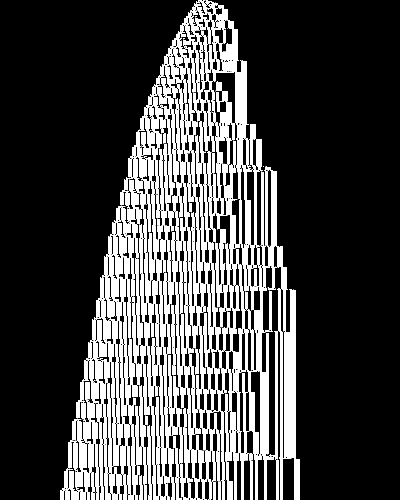
\includegraphics[scale=0.35]{figures/bouncers/5608043.png}
    \caption{\small 50,000-step space-time diagram of \url{https://bbchallenge.org/5608043}. Out of the 29,799 decided bouncers, this bouncer takes the most steps (141,509) to be detected and fits the biggest formula tape (378 0/1 symbols), using the method presented in this section.}\label{fig:big-bounce}
\end{figure}
\vspace{-2.5ex}
\paragraph*{Remarkable bouncers.} Out of the 29,799 bouncers that were decided using the method presented in this section, here are some remarkable facts:
\begin{enumerate}
    \item Only two bouncers have 3 repeaters and that's the maximum: \url{https://bbchallenge.org/347505} and \url{https://bbchallenge.org/8131743}. Otherwise, 2132 bouncers have 2 repeaters and the rest has only 1.
    \item\label{pt:big-formula-tape} The biggest fitted formula tapes by the algorithm (but note that formulas are not necessarily minimal, see Remark~\ref{rk:minimal-formula-tapes}) have 378 symbols (summing walls and repeater symbols), there are two of them, such as for machine \url{https://bbchallenge.org/5608043}, see Figure~\ref{fig:big-bounce}:
          \begin{align*}
               & 0^\infty\lhead{\text{A}} 1000001110001110000001110000111011100111011100111000011100 0011101110011100001110
              \\ &1110011101110011100001110000111011100111000011100001110000111000011101110011101110011\\ &1011100111011100111011100111011100111011100111011100111011100111011100 (111011100111011\\
               & 100111011100111011100)000111000011100000011100111111111111111
              0000111111111111111(11111                                                                                     \\ &1111111)                                                                            001110000000111000000111111001111110^\infty
          \end{align*}

    \item The above machine of Point~\ref{pt:big-formula-tape} is also the machine that is detected after the most steps: 141,509. Over this dataset, it took 202 steps on average.
    \item The most macro steps (i.e.\ number of usual or shift rule steps in formula tape simulation) needed to conclude using Theorem~\ref{th:bouncers} was 44,898 for \url{https://bbchallenge.org/347505}. Otherwise, it took 107 macro steps on average.

\end{enumerate}
